\documentclass[11pt]{article}

\usepackage[margin=1in]{geometry}
\usepackage{graphicx}
\usepackage{booktabs}
\usepackage{float}
\usepackage{amsmath}
\usepackage{caption}
\usepackage{xcolor}
\usepackage{hyperref}
\usepackage{tikz}
\usetikzlibrary{arrows.meta,positioning}

\definecolor{diagramblue}{HTML}{1F4E79}
\definecolor{diagramlight}{HTML}{EAF2F8}
\definecolor{diagramgray}{HTML}{F2F4F4}
\tikzset{
  diagram node/.style={draw=diagramblue, rounded corners=2pt,
    fill=diagramlight, text width=2.15cm, minimum height=0.78cm,
    align=center, font=\small},
  diagram process/.style={draw=black!45, rounded corners=2pt,
    fill=diagramgray, text width=2.15cm, minimum height=0.78cm,
    align=center, font=\small},
  diagram arrow/.style={-{Latex[length=2mm]}, draw=black!65, line width=0.7pt}
}

\hypersetup{
  pdftitle={EN3150 Assignment 03 - Resource-Constrained CNN for Edge Image Classification},
  pdfauthor={EN3150 Assignment 03 Group}
}

\title{EN3150 Assignment 03 \\ \large Resource-Constrained CNN for Edge Image Classification}
\author{
  S.E.N. Silva (230615V) \\
  R.P.M. Vithanage (230674A) \\
  S.V.C.H. Vithanage (230675D) \\[0.5em]
  GitHub repository: \url{https://github.com/rash200319/CNN-for-image-classification}
}
\date{\today}

\begin{document}
\begin{titlepage}
\thispagestyle{empty}
\centering
\vspace*{1.5cm}

{\Large\textsc{EN3150 Assignment 03}\par}
\vspace{1.2cm}
{\Huge\bfseries Resource Constrained CNN\par}
\vspace{0.25cm}
{\Huge\bfseries for Edge Image Classification\par}
\vspace{1.4cm}

{\large\textcolor{diagramblue}{EuroSAT land use classification study}\par}
\vfill

\begin{table}[H]
\centering
\caption*{\large\textbf{Group members}}
\renewcommand{\arraystretch}{1.35}
\begin{tabular}{|p{1.65in}|c|p{3.15in}|}
\hline
\textbf{Name} & \textbf{Index number} & \textbf{Contribution} \\
\hline
S.E.N. Silva & 230615V & Model design and experimentation \\
\hline
R.P.M. Vithanage & 230674A & Training and evaluation pipeline \\
\hline
S.V.C.H. Vithanage & 230675D & Analysis and report preparation \\
\hline
\end{tabular}
\end{table}

\vspace{1cm}
\begin{tabular}{rl}
\textbf{Course:} & EN3150 \\
\textbf{Dataset:} & EuroSAT RGB \\
\textbf{Repository:} &
\url{github.com/rash200319/CNN-for-image-classification} \\
\textbf{Date:} & \today
\end{tabular}

\vfill
{\small Department of Computer Engineering\par}
\end{titlepage}

\pagenumbering{roman}
\tableofcontents
\clearpage
\pagenumbering{arabic}

\section{Data Preparation}

\subsection{Dataset}
This work uses the RGB variant of the \textbf{EuroSAT} land use/land cover
dataset, which consists of 27{,}000 Sentinel 2 satellite image patches of
size $64 \times 64$ pixels across 10 approximately balanced classes:
AnnualCrop, Forest, HerbaceousVegetation, Highway, Industrial, Pasture,
PermanentCrop, Residential, River, and SeaLake. Because the images are already at
$64\times64$ resolution, no downscaling was required to satisfy the
assignment's maximum resolution constraint; both custom models and both
pretrained SOTA models are trained and evaluated at $64\times64$ to strictly
comply with the assignment's maximum resolution requirement.

\begin{figure}[H]
\centering
\renewcommand{\arraystretch}{0.9}
\begin{tabular}{ccccc}
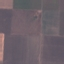
\includegraphics[width=0.17\textwidth]{figures/eurosat_AnnualCrop.jpg} &
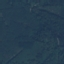
\includegraphics[width=0.17\textwidth]{figures/eurosat_Forest.jpg} &
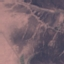
\includegraphics[width=0.17\textwidth]{figures/eurosat_HerbaceousVegetation.jpg} &
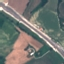
\includegraphics[width=0.17\textwidth]{figures/eurosat_Highway.jpg} &
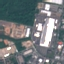
\includegraphics[width=0.17\textwidth]{figures/eurosat_Industrial.jpg} \\
\scriptsize AnnualCrop & \scriptsize Forest &
\scriptsize Herbaceous vegetation & \scriptsize Highway &
\scriptsize Industrial \\[0.6em]
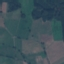
\includegraphics[width=0.17\textwidth]{figures/eurosat_Pasture.jpg} &
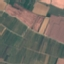
\includegraphics[width=0.17\textwidth]{figures/eurosat_PermanentCrop.jpg} &
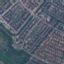
\includegraphics[width=0.17\textwidth]{figures/eurosat_Residential.jpg} &
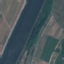
\includegraphics[width=0.17\textwidth]{figures/eurosat_River.jpg} &

\includegraphics[width=0.17\textwidth]{figures/eurosat_SeaLake.jpg} \\
\scriptsize Pasture & \scriptsize Permanent crop &
\scriptsize Residential & \scriptsize River & \scriptsize Sea/lake
\end{tabular}
\caption{One representative RGB image from each EuroSAT class. The labels
identify the target class; the examples are intended to illustrate the
visual cues available to the classifier rather than define the classes
exhaustively.}
\label{fig:eurosat-class-overview}
\end{figure}

The classes are separated mainly by spatial arrangement, texture, colour,
and the presence of human-made structures. The most useful visual cues and
common sources of confusion are summarized in Table~\ref{tab:class-cues}.

\begin{table}[H]
\centering
\caption{Distinctive visual cues and likely confusions between EuroSAT
classes.}
\label{tab:class-cues}
\small
\renewcommand{\arraystretch}{1.18}
\begin{tabular}{|p{1.35in}|p{2.55in}|p{2.25in}|}
\hline
\textbf{Class} & \textbf{Distinctive separable cues} & \textbf{Likely confusion} \\
\hline
AnnualCrop & Large, regular cultivated fields with seasonal bare soil or crop patterns. & PermanentCrop; Pasture \\
\hline
Forest & Dense, continuous tree canopy with fine, irregular texture. & HerbaceousVegetation; Pasture \\
\hline
HerbaceousVegetation & Open green cover with coarse, irregular natural texture and few field boundaries. & Forest; Pasture \\
\hline
Highway & Long, narrow linear road surfaces, junctions, and surrounding verges. & River; Residential \\
\hline
Industrial & Large bright roofs, warehouses, paved yards, and rectilinear layouts. & Residential; Highway \\
\hline
Pasture & Open grassland with relatively uniform green cover and fewer crop boundaries. & HerbaceousVegetation; AnnualCrop \\
\hline
PermanentCrop & Repeated orchard or plantation rows with regular spacing. & AnnualCrop; Forest \\
\hline
Residential & Dense clusters of buildings, roads, and small fragmented plots. & Industrial; Highway \\
\hline
River & Winding, narrow water corridor with visible banks and surrounding vegetation. & Highway; Sea/lake \\
\hline
SeaLake & Broad, contiguous water body with large smooth dark or blue regions. & River \\
\hline
\end{tabular}
\end{table}

\subsection{Train / Validation / Test split}
The dataset was split \textbf{70\% / 15\% / 15\%} into training, validation,
and test sets using a stratified split (per class proportions preserved) with
a fixed random seed (42) for reproducibility. This gives approximately
18{,}900 training, 4{,}050 validation, and 4{,}050 test images; exact
per class counts vary by at most one or two images due to stratified
rounding.

\subsection{Preprocessing and augmentation}
All images were normalized per channel. For the two custom models
(Section~\ref{sec:custom-models}), pixel values were normalized with
mean $=$ std $= 0.5$ per channel (mapping to the $[-1, 1]$ range), and the
training split was augmented with random horizontal and vertical flips
(satellite imagery has no canonical orientation, so both flips are valid
label-preserving augmentations). The validation and test splits use the same
resizing and normalization but no augmentation. For the pretrained models,
ImageNet normalization statistics ($\mu = [0.485, 0.456, 0.406]$,
$\sigma = [0.229, 0.224, 0.225]$) were used instead, matching what those
networks were originally trained with.

The dataset information sheet was completed and checked against the RGB
EuroSAT dataset used in this work.

\subsection{Pipeline overview}

Figure~\ref{fig:data-pipeline} summarizes the data preparation pipeline
described above, from raw images to model-ready batches.

\begin{figure}[H]
\centering
\resizebox{0.92\textwidth}{!}{%
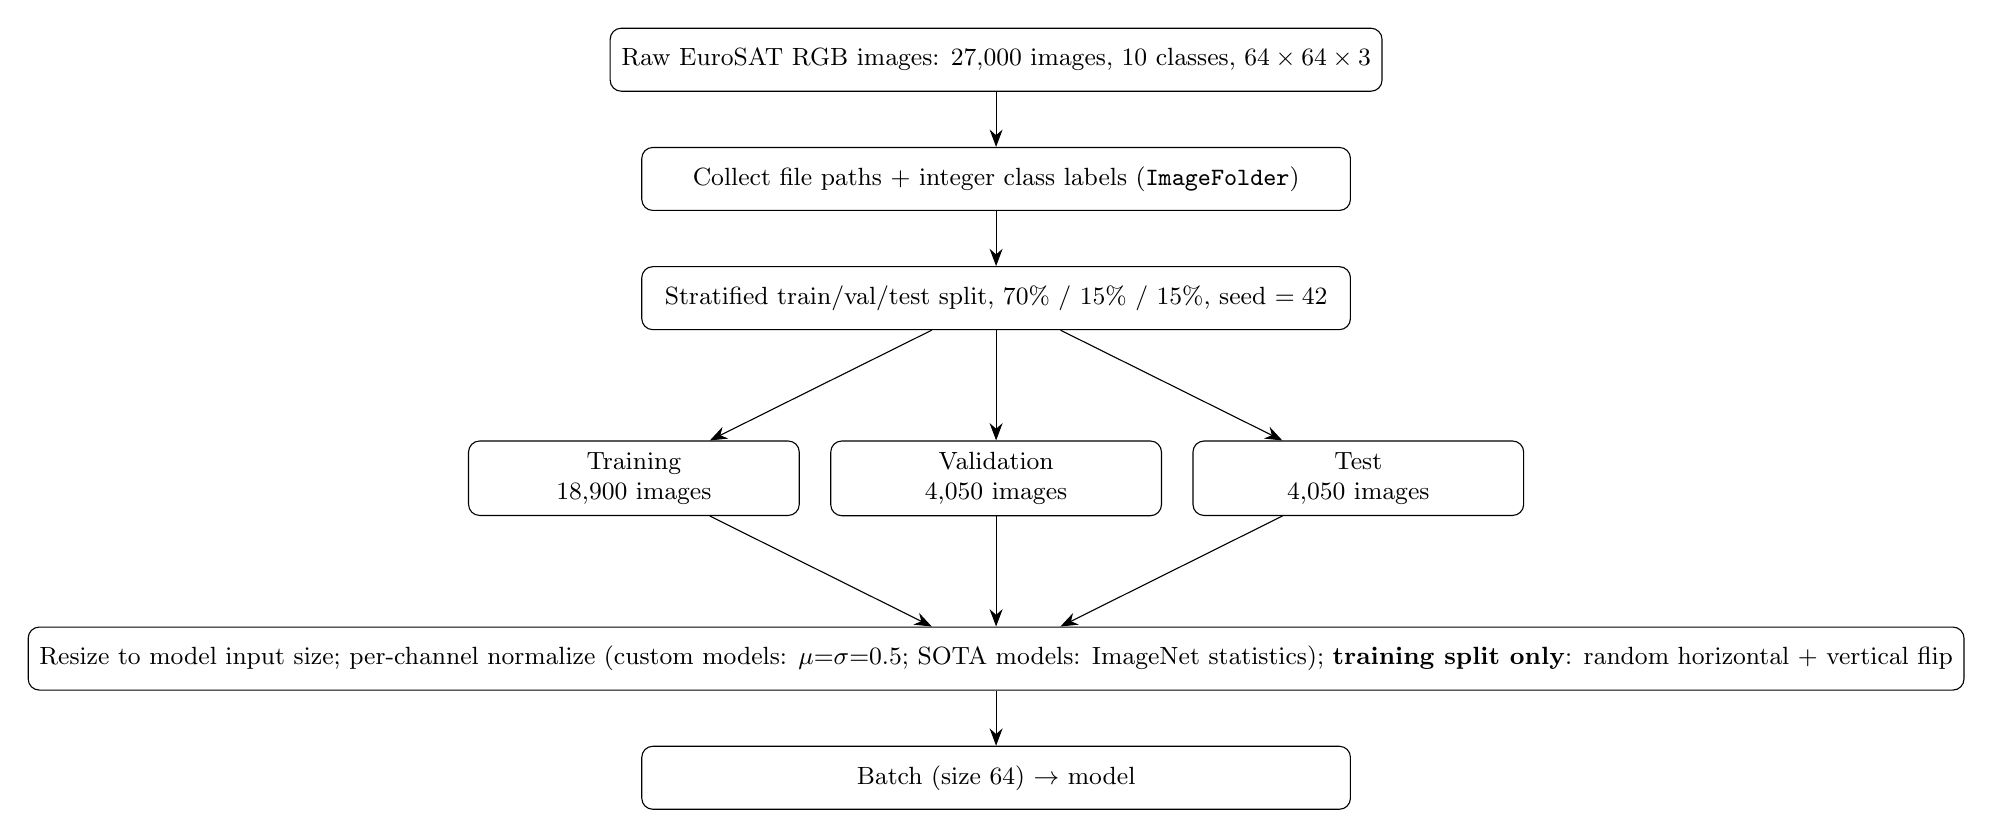
\begin{tikzpicture}[
  node distance=7mm and 10mm,
  box/.style={draw, rounded corners, align=center, font=\small, minimum height=8mm, inner sep=4pt},
  wide/.style={box, minimum width=9cm},
  narrow/.style={box, minimum width=4.2cm},
  arr/.style={-{Stealth[length=2.2mm]}}
]
\node[wide] (raw) {Raw EuroSAT RGB images: 27{,}000 images, 10 classes, $64\times64\times3$};
\node[wide, below=of raw] (paths) {Collect file paths + integer class labels (\texttt{ImageFolder})};
\node[wide, below=of paths] (split) {Stratified train/val/test split, 70\% / 15\% / 15\%, seed $=42$};
\node[narrow, below=14mm of split, xshift=-4.6cm] (train) {Training\\18{,}900 images};
\node[narrow, below=14mm of split] (val) {Validation\\4{,}050 images};
\node[narrow, below=14mm of split, xshift=4.6cm] (test) {Test\\4{,}050 images};
\node[wide, below=14mm of val] (prep) {Resize to model input size; per-channel normalize (custom models: $\mu{=}\sigma{=}0.5$; SOTA models: ImageNet statistics); \textbf{training split only}: random horizontal + vertical flip};
\node[wide, below=of prep] (batch) {Batch (size 64) $\rightarrow$ model};

\draw[arr] (raw) -- (paths);
\draw[arr] (paths) -- (split);
\draw[arr] (split) -- (train);
\draw[arr] (split) -- (val);
\draw[arr] (split) -- (test);
\draw[arr] (train) -- (prep);
\draw[arr] (val) -- (prep);
\draw[arr] (test) -- (prep);
\draw[arr] (prep) -- (batch);
\end{tikzpicture}%
}
\caption{Data preparation and preprocessing pipeline.}
\label{fig:data-pipeline}
\end{figure}

\begin{figure}[H]
\centering
\resizebox{\linewidth}{!}{%
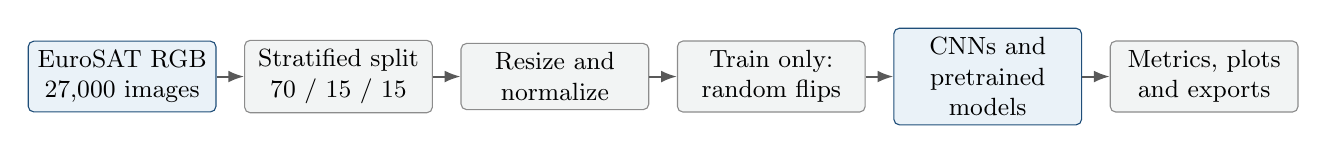
\begin{tikzpicture}[node distance=0.25cm and 0.35cm]
  \node[diagram node] (data) {EuroSAT RGB\\27,000 images};
  \node[diagram process, right=of data] (split) {Stratified split\\70 / 15 / 15};
  \node[diagram process, right=of split] (prep) {Resize and\\normalize};
  \node[diagram process, right=of prep] (aug) {Train only:\\random flips};
  \node[diagram node, right=of aug] (models) {CNNs and\\pretrained models};
  \node[diagram process, right=of models] (eval) {Metrics, plots\\and exports};
  \draw[diagram arrow] (data) -- (split);
  \draw[diagram arrow] (split) -- (prep);
  \draw[diagram arrow] (prep) -- (aug);
  \draw[diagram arrow] (aug) -- (models);
  \draw[diagram arrow] (models) -- (eval);
\end{tikzpicture}}
\caption{End to end experimental pipeline. Augmentation is applied only to
the training split; validation and test images remain deterministic.}
\label{fig:experimental-pipeline}
\end{figure}

\section{Custom Architecture Design}
\label{sec:custom-models}

Both custom models follow the standard CNN pipeline:
\texttt{[Conv + ReLU] → Pool → [Conv + ReLU] → Pool → ... → Classifier →
Softmax}, taking a $3 \times 64 \times 64$ RGB input and producing a
10-class prediction. The shared data and evaluation flow is summarized in
Figure~\ref{fig:experimental-pipeline}.

\begin{figure}[H]
\centering
\resizebox{0.88\linewidth}{!}{%
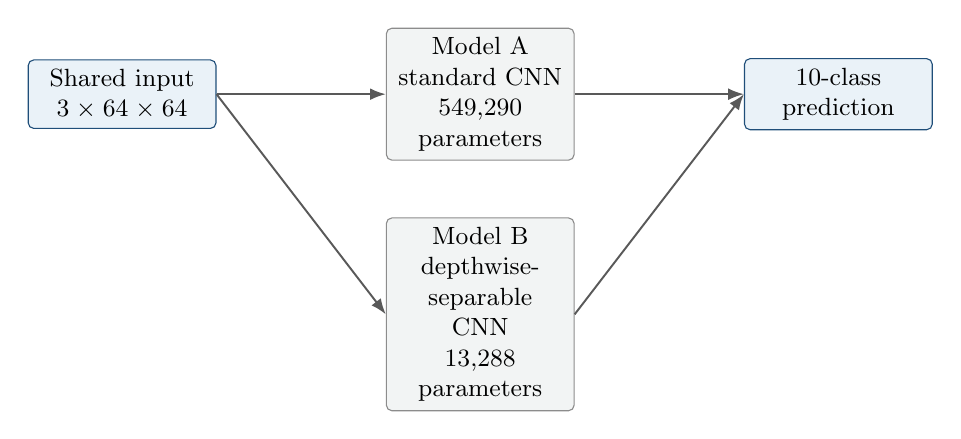
\begin{tikzpicture}[node distance=0.42cm and 0.9cm]
  \node[diagram node] (input) {Shared input\\$3\times64\times64$};
  \node[diagram process, right=2.15cm of input] (a)
    {Model A\\standard CNN\\549,290 parameters};
  \node[diagram process, below=0.72cm of a] (b)
    {Model B\\depthwise-separable CNN\\13,288 parameters};
  \node[diagram node, right=2.15cm of a] (output) {10-class\\prediction};
  \draw[diagram arrow] (input.east) -- (a.west);
  \draw[diagram arrow] (input.east) -- (b.west);
  \draw[diagram arrow] (a.east) -- (output.west);
  \draw[diagram arrow] (b.east) -- (output.west);
\end{tikzpicture}}
\caption{Custom architecture design overview. Both models use the same
$64\times64$ RGB input and ten-class output, but differ in their feature
extraction and classifier design.}
\label{fig:custom-architecture-overview}
\end{figure}

\subsection{Model A: Standard CNN}

Model A interleaves regular 2D convolutions with max-pooling layers,
followed by a flatten and two fully-connected layers, as shown in
Figure~\ref{fig:model-a-pipeline}.

\begin{figure}[H]
\centering
\resizebox{\linewidth}{!}{%
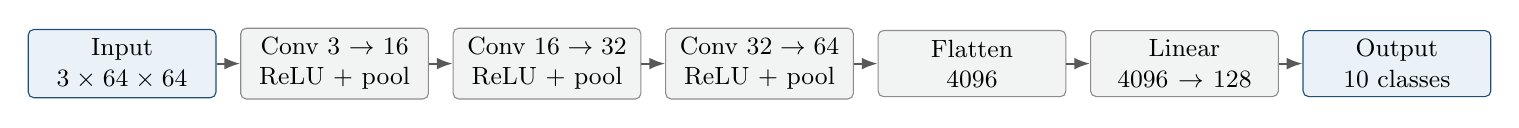
\begin{tikzpicture}[node distance=0.25cm and 0.3cm]
  \node[diagram node] (input) {Input\\$3\times64\times64$};
  \node[diagram process, right=of input] (c1) {Conv $3\to16$\\ReLU + pool};
  \node[diagram process, right=of c1] (c2) {Conv $16\to32$\\ReLU + pool};
  \node[diagram process, right=of c2] (c3) {Conv $32\to64$\\ReLU + pool};
  \node[diagram process, right=of c3] (flat) {Flatten\\$4096$};
  \node[diagram process, right=of flat] (fc) {Linear\\$4096\to128$};
  \node[diagram node, right=of fc] (out) {Output\\10 classes};
  \draw[diagram arrow] (input) -- (c1);
  \draw[diagram arrow] (c1) -- (c2);
  \draw[diagram arrow] (c2) -- (c3);
  \draw[diagram arrow] (c3) -- (flat);
  \draw[diagram arrow] (flat) -- (fc);
  \draw[diagram arrow] (fc) -- (out);
\end{tikzpicture}}
\caption{Model A forward path. Three standard convolution stages are followed
by a parameter-heavy flattened classifier head.}
\label{fig:model-a-pipeline}
\end{figure}

\begin{table}[H]
\centering
\caption{Model A architecture.}
\label{tab:model-a-arch}
\begin{tabular}{lll}
\toprule
Layer & Configuration & Output shape \\
\midrule
Input & -- & $3 \times 64 \times 64$ \\
Conv2D + ReLU & $16$ filters, $3\times3$, pad 1 & $16 \times 64 \times 64$ \\
MaxPool2D & $2\times2$ & $16 \times 32 \times 32$ \\
Conv2D + ReLU & $32$ filters, $3\times3$, pad 1 & $32 \times 32 \times 32$ \\
MaxPool2D & $2\times2$ & $32 \times 16 \times 16$ \\
Conv2D + ReLU & $64$ filters, $3\times3$, pad 1 & $64 \times 16 \times 16$ \\
MaxPool2D & $2\times2$ & $64 \times 8 \times 8$ \\
Flatten & -- & $4096$ \\
Linear + ReLU & $4096 \rightarrow 128$ & $128$ \\
Linear & $128 \rightarrow 10$ & $10$ \\
\bottomrule
\end{tabular}
\end{table}

\paragraph{Calculated parameter count.} For a standard Conv2D layer the
trainable parameter count is $C_{out} \cdot C_{in} \cdot K^2 + C_{out}$ (the
$+C_{out}$ term is the bias), and for a Linear layer it is
$\text{in} \cdot \text{out} + \text{out}$.

\begin{table}[H]
\centering
\caption{Model A parameter breakdown.}
\label{tab:model-a-params}
\begin{tabular}{lrr}
\toprule
Layer & Formula & Parameters \\
\midrule
Conv1 ($3 \rightarrow 16$) & $16 \cdot 3 \cdot 3^2 + 16$ & 448 \\
Conv2 ($16 \rightarrow 32$) & $32 \cdot 16 \cdot 3^2 + 32$ & 4{,}640 \\
Conv3 ($32 \rightarrow 64$) & $64 \cdot 32 \cdot 3^2 + 64$ & 18{,}496 \\
FC1 ($4096 \rightarrow 128$) & $4096 \cdot 128 + 128$ & 524{,}416 \\
FC2 ($128 \rightarrow 10$) & $128 \cdot 10 + 10$ & 1{,}290 \\
\midrule
\textbf{Total} & & \textbf{549{,}290} \\
\bottomrule
\end{tabular}
\end{table}

Note that FC1 alone accounts for $524{,}416 / 549{,}290 \approx 95.5\%$ of
the model's parameters: flattening an $8\times8\times64$ feature map into a
128 unit fully connected layer is by far the most expensive operation in
this architecture, far more costly than any of the convolutional layers.
This observation motivates Model B's design (global average pooling instead
of a large flatten + FC head). The hand-calculated total of 549{,}290 was
cross checked against a runtime parameter count
(\texttt{sum(p.numel() for p in model.parameters())}) and matches exactly.

\subsection{Model B: Lightweight depthwise separable CNN}

Model B replaces every standard convolution with a \textbf{depthwise
separable convolution}: a depthwise $K \times K$ convolution applied
independently per input channel (no cross channel mixing), followed by a
$1\times1$ pointwise convolution that mixes channels. This is the
construction used in MobileNet style architectures, and it reduces the
multiply accumulate (MAC) cost of a $3\times3$ convolution by roughly a
factor of $K^2 \cdot C_{out} / (K^2 + C_{out})$ (around $8$--$9\times$ for
typical layer widths) relative to a full standard convolution of the same
shape. Each depthwise separable block is followed by batch normalization and
ReLU. The classifier head uses global average pooling (GAP) instead of a
flatten, which is the main reason Model B's parameter count stays small.
The resulting forward path is shown in Figure~\ref{fig:model-b-pipeline}.

\begin{figure}[H]
\centering
\resizebox{\linewidth}{!}{%
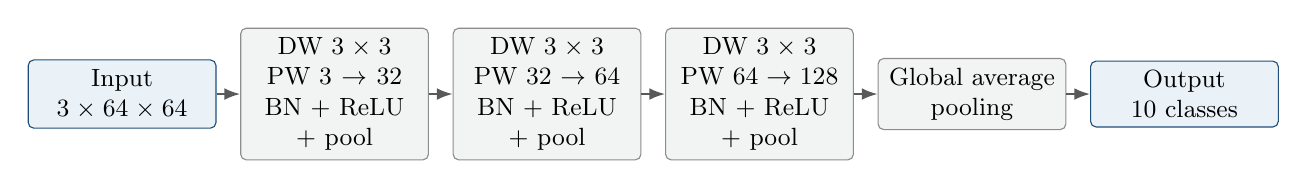
\begin{tikzpicture}[node distance=0.25cm and 0.3cm]
  \node[diagram node] (input) {Input\\$3\times64\times64$};
  \node[diagram process, right=of input] (b1) {DW $3\times3$\\PW $3\to32$\\BN + ReLU + pool};
  \node[diagram process, right=of b1] (b2) {DW $3\times3$\\PW $32\to64$\\BN + ReLU + pool};
  \node[diagram process, right=of b2] (b3) {DW $3\times3$\\PW $64\to128$\\BN + ReLU + pool};
  \node[diagram process, right=of b3] (gap) {Global average\\pooling};
  \node[diagram node, right=of gap] (out) {Output\\10 classes};
  \draw[diagram arrow] (input) -- (b1);
  \draw[diagram arrow] (b1) -- (b2);
  \draw[diagram arrow] (b2) -- (b3);
  \draw[diagram arrow] (b3) -- (gap);
  \draw[diagram arrow] (gap) -- (out);
\end{tikzpicture}}
\caption{Model B forward path. Each depthwise-separable stage combines
depthwise convolution, pointwise channel mixing and batch normalization;
the pooling layers follow each stage, and global average pooling avoids a
large flatten layer.}
\label{fig:model-b-pipeline}
\end{figure}

\begin{table}[H]
\centering
\caption{Model B architecture.}
\label{tab:model-b-arch}
\begin{tabular}{lll}
\toprule
Layer & Configuration & Output shape \\
\midrule
Input & -- & $3 \times 64 \times 64$ \\
DWSepConv + BN + ReLU & $3 \rightarrow 32$, $3\times3$ & $32 \times 64 \times 64$ \\
MaxPool2D & $2\times2$ & $32 \times 32 \times 32$ \\
DWSepConv + BN + ReLU & $32 \rightarrow 64$, $3\times3$ & $64 \times 32 \times 32$ \\
MaxPool2D & $2\times2$ & $64 \times 16 \times 16$ \\
DWSepConv + BN + ReLU & $64 \rightarrow 128$, $3\times3$ & $128 \times 16 \times 16$ \\
MaxPool2D & $2\times2$ & $128 \times 8 \times 8$ \\
AdaptiveAvgPool2D & output $1\times1$ & $128 \times 1 \times 1$ \\
Linear & $128 \rightarrow 10$ & $10$ \\
\bottomrule
\end{tabular}
\end{table}

\paragraph{Calculated parameter count.} A depthwise conv (groups $=
C_{in}$, one filter per channel) costs $C_{in} \cdot K^2 + C_{in}$; a
pointwise $1\times1$ conv costs $C_{in} \cdot C_{out} + C_{out}$; and a
BatchNorm2D layer contributes $2C$ learnable parameters (scale $\gamma$ and
shift $\beta$ only : the running mean/variance are buffers, not trainable
parameters).

\begin{table}[H]
\centering
\caption{Model B parameter breakdown.}
\label{tab:model-b-params}
\begin{tabular}{lrr}
\toprule
Layer & Formula & Parameters \\
\midrule
DWSepConv1 depthwise ($3$ ch) & $3 \cdot 3^2 + 3$ & 30 \\
DWSepConv1 pointwise ($3 \rightarrow 32$) & $3 \cdot 32 + 32$ & 128 \\
DWSepConv1 BatchNorm ($32$ ch) & $2 \cdot 32$ & 64 \\
DWSepConv2 depthwise ($32$ ch) & $32 \cdot 3^2 + 32$ & 320 \\
DWSepConv2 pointwise ($32 \rightarrow 64$) & $32 \cdot 64 + 64$ & 2{,}112 \\
DWSepConv2 BatchNorm ($64$ ch) & $2 \cdot 64$ & 128 \\
DWSepConv3 depthwise ($64$ ch) & $64 \cdot 3^2 + 64$ & 640 \\
DWSepConv3 pointwise ($64 \rightarrow 128$) & $64 \cdot 128 + 128$ & 8{,}320 \\
DWSepConv3 BatchNorm ($128$ ch) & $2 \cdot 128$ & 256 \\
Classifier ($128 \rightarrow 10$) & $128 \cdot 10 + 10$ & 1{,}290 \\
\midrule
\textbf{Total} & & \textbf{13{,}288} \\
\bottomrule
\end{tabular}
\end{table}

This is well within the assignment's 100{,}000 parameter budget for Model B,
using only $13.3\%$ of it ($86.7\%$ headroom). This headroom is a deliberate
consequence of the GAP based head rather than an accident: a flatten of the
final $8\times8\times128$ feature map into even a modestly sized FC layer
would alone cost well over $100{,}000$ parameters, so GAP was essential to
the design, not an afterthought. The hand calculated total was likewise
cross checked against a runtime parameter count and matches exactly.

\subsection{Activation function justification}
Both models use \textbf{ReLU} ($f(x) = \max(0, x)$) exclusively as the
nonlinearity, rather than sigmoid or tanh. This is justified on
hardware efficiency grounds, which matters directly for the
resource constrained/edge deployment target of this assignment:
\begin{itemize}
  \item ReLU requires only a single comparison and a conditional select per
  element, with no transcendental (exponential) function evaluation. Sigmoid
  and tanh both require computing $e^{-x}$, which is substantially more
  expensive on microcontroller class hardware that lacks a dedicated
  floating point transcendental unit.
  \item ReLU's gradient is either $0$ or $1$, which is cheap to compute
  during backpropagation and avoids the vanishing gradient problem that
  sigmoid/tanh exhibit for large $|x|$.
  \item ReLU activations are naturally sparse (exactly zero for negative
  inputs), which many inference engines and accelerators can exploit to skip
  computation.
\end{itemize}

\section{Optimizer Selection and Tuning}
\label{sec:optimizer}

\textbf{Adam with a learning rate of $1\times10^{-3}$} was selected as the
optimizer for the final training runs of both custom models. Adam was
chosen because it adapts the effective learning rate per parameter using
running estimates of the first and second gradient moments, which typically
gives faster and more reliable convergence than plain SGD without requiring
extensive learning-rate tuning : a useful property given the limited
CPU only compute budget available for this assignment.

\subsection{Comparison against SGD and SGD with Momentum}

Two independent experiments were run to justify this choice.

\paragraph{Model A, 10 epoch sweep.} Adam ($\text{lr}=10^{-3}$), plain SGD
($\text{lr}=10^{-2}$), and SGD with momentum ($\text{lr}=10^{-2}$,
$\text{momentum}=0.9$) were each trained for 10 epochs. SGD and SGD+momentum
were given the same (larger) learning rate since, without adaptive scaling,
SGD needs a bigger step to make comparable progress in the same number of
epochs; momentum's effect can then be isolated cleanly since the learning
rate is held fixed between the two SGD variants.

\begin{table}[H]
\centering
\caption{Model A optimizer sweep, validation accuracy/loss after 10 epochs.}
\label{tab:model-a-sweep}
\begin{tabular}{lrrrr}
\toprule
Optimizer & LR & Train acc. & Val. acc. & Val. loss \\
\midrule
Adam & $10^{-3}$ & 87.0\% & 83.1\% & 0.484 \\
SGD & $10^{-2}$ & 62.2\% & 46.5\% & 1.520 \\
SGD + Momentum (0.9) & $10^{-2}$ & 87.2\% & 83.7\% & 0.484 \\
\bottomrule
\end{tabular}
\end{table}

\begin{figure}[H]
\centering
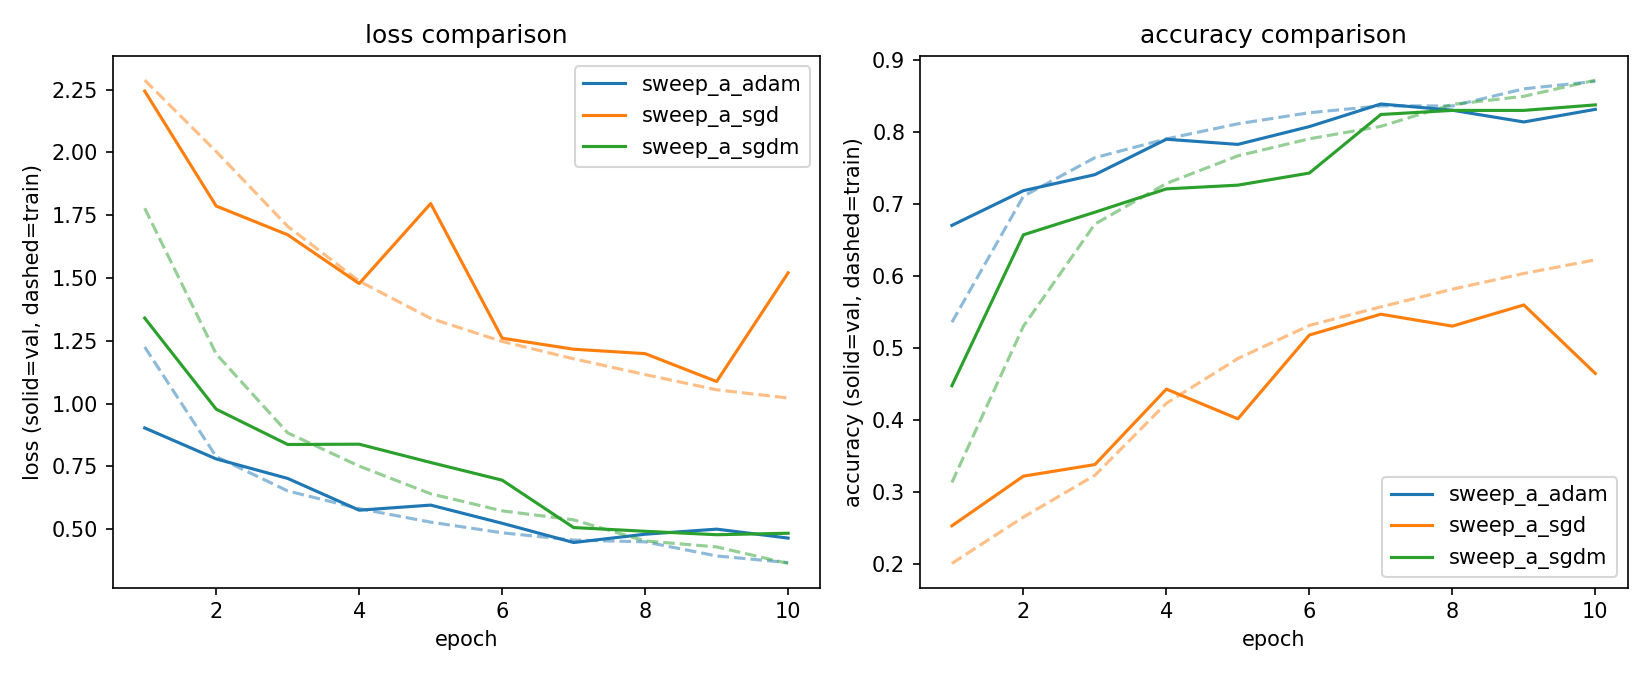
\includegraphics[width=0.95\textwidth]{figures/model_a_optimizer_sweep.png}
\caption{Model A optimizer sweep: validation (solid) and training (dashed)
loss and accuracy vs. epoch, for Adam, plain SGD, and SGD with momentum.}
\label{fig:model-a-sweep}
\end{figure}

\paragraph{Model B, full 20 epoch runs.} As a second, independent
confirmation, Model B was trained to completion (20 epochs, test set
evaluated) under all three optimizer settings.

\begin{table}[H]
\centering
\caption{Model B optimizer comparison, full 20 epoch test set results.}
\label{tab:model-b-optimizer}
\begin{tabular}{lrrr}
\toprule
Optimizer & Test accuracy & Macro precision & Macro recall \\
\midrule
Adam & \textbf{91.01\%} & 0.9087 & 0.9064 \\
SGD & 79.88\% & 0.7967 & 0.7879 \\
SGD + Momentum (0.9) & 89.90\% & 0.8963 & 0.8968 \\
\bottomrule
\end{tabular}
\end{table}

\paragraph{Discussion: effect of momentum.} In both experiments, plain SGD
is clearly the weakest optimizer : its validation loss is both higher and
visibly less stable (Figure~\ref{fig:model-a-sweep} shows a sharp spike
around epoch 5), and on Model B it is $11.13$ percentage points behind
Adam in test accuracy ($79.88\%$ vs.\ $91.01\%$). Adding momentum (velocity term $v_{t} = \mu v_{t-1} +
\nabla_\theta \mathcal{L}$, with the parameter update using $v_t$ instead of
the raw gradient) at the \emph{same} learning rate dramatically changes this
picture: the momentum term accumulates an exponentially weighted average of
past gradients, which (i) damps oscillation in directions where the gradient
sign repeatedly flips, and (ii) effectively increases the step size in
directions where the gradient is consistently pointing the same way. This is
exactly what is observed here : SGD with momentum converges significantly faster
than plain SGD (+$10.02$ percentage points) and closes nearly the entire accuracy gap,
reaching $89.90\%$ test accuracy (within $1.11$ percentage points of Adam on Model B,
and ahead of Adam on the Model A sweep by epoch 10), despite using a much simpler update rule.
This confirms that most of the practical convergence benefit over plain SGD in this setting comes
from momentum specifically, rather than from Adam's additional per parameter
adaptive scaling.

\section{Custom Model Training and Evaluation}
\label{sec:custom-training}

Both Model A and Model B were trained for 20 epochs using Adam
($\text{lr}=10^{-3}$), as justified in Section~\ref{sec:optimizer}. The same
training, evaluation, and comparison pipeline (Figure~\ref{fig:training-pipeline})
was used for all four models reported in this document, so that figures and
tables can be regenerated directly from saved run artifacts rather than
copied by hand.

\begin{figure}[H]
\centering
\resizebox{0.92\textwidth}{!}{%
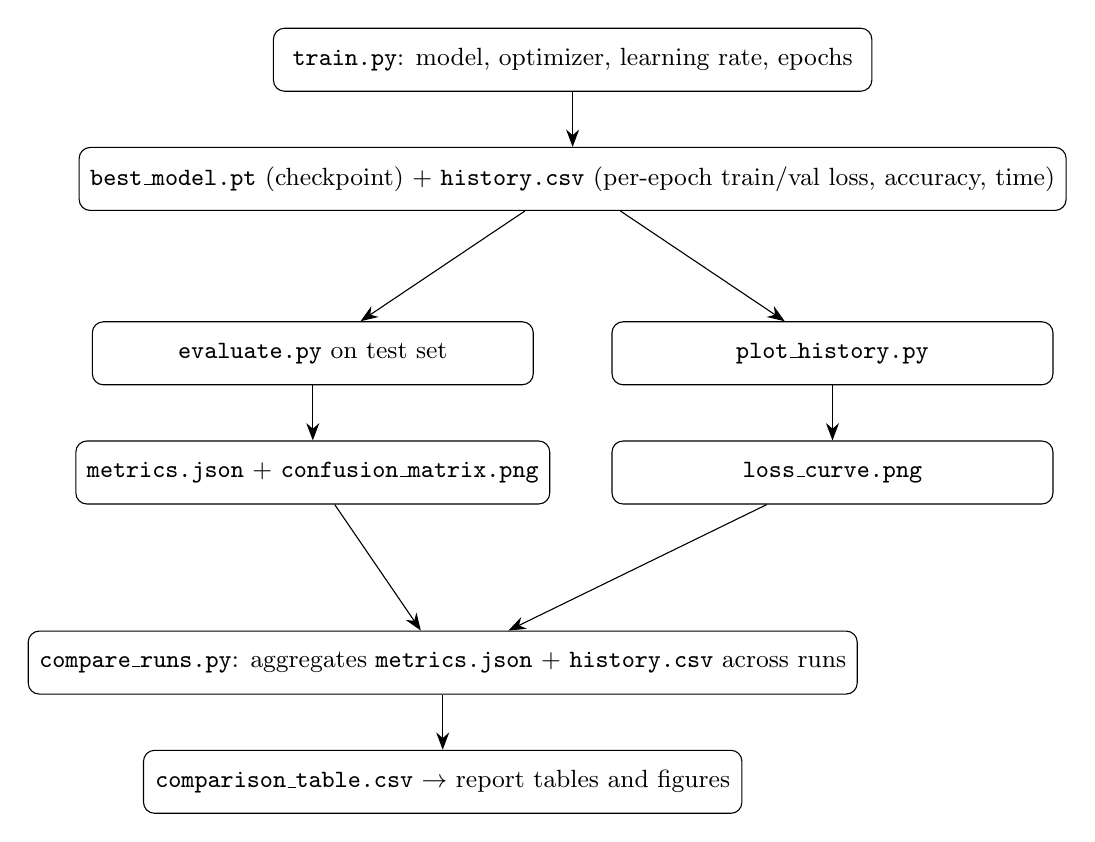
\begin{tikzpicture}[
  node distance=7mm and 10mm,
  box/.style={draw, rounded corners, align=center, font=\small, minimum height=8mm, inner sep=4pt},
  wide/.style={box, minimum width=7.6cm},
  narrow/.style={box, minimum width=5.6cm},
  arr/.style={-{Stealth[length=2.2mm]}}
]
\node[wide] (train) {\texttt{train.py}: model, optimizer, learning rate, epochs};
\node[wide, below=of train] (ckpt) {\texttt{best\_model.pt} (checkpoint) + \texttt{history.csv} (per-epoch train/val loss, accuracy, time)};
\node[narrow, below=14mm of ckpt, xshift=-3.3cm] (eval) {\texttt{evaluate.py} on test set};
\node[narrow, below=14mm of ckpt, xshift=3.3cm] (plot) {\texttt{plot\_history.py}};
\node[narrow, below=of eval] (evalout) {\texttt{metrics.json} + \texttt{confusion\_matrix.png}};
\node[narrow, below=of plot] (plotout) {\texttt{loss\_curve.png}};
\node[wide, below=16mm of evalout, xshift=1.65cm] (compare) {\texttt{compare\_runs.py}: aggregates \texttt{metrics.json} + \texttt{history.csv} across runs};
\node[wide, below=of compare] (table) {\texttt{comparison\_table.csv} $\rightarrow$ report tables and figures};

\draw[arr] (train) -- (ckpt);
\draw[arr] (ckpt) -- (eval);
\draw[arr] (ckpt) -- (plot);
\draw[arr] (eval) -- (evalout);
\draw[arr] (plot) -- (plotout);
\draw[arr] (evalout) -- (compare);
\draw[arr] (plotout) -- (compare);
\draw[arr] (compare) -- (table);
\end{tikzpicture}%
}
\caption{Training, evaluation, and comparison pipeline, shared by all four models.}
\label{fig:training-pipeline}
\end{figure}

\begin{figure}[H]
\centering
\resizebox{0.92\textwidth}{!}{%
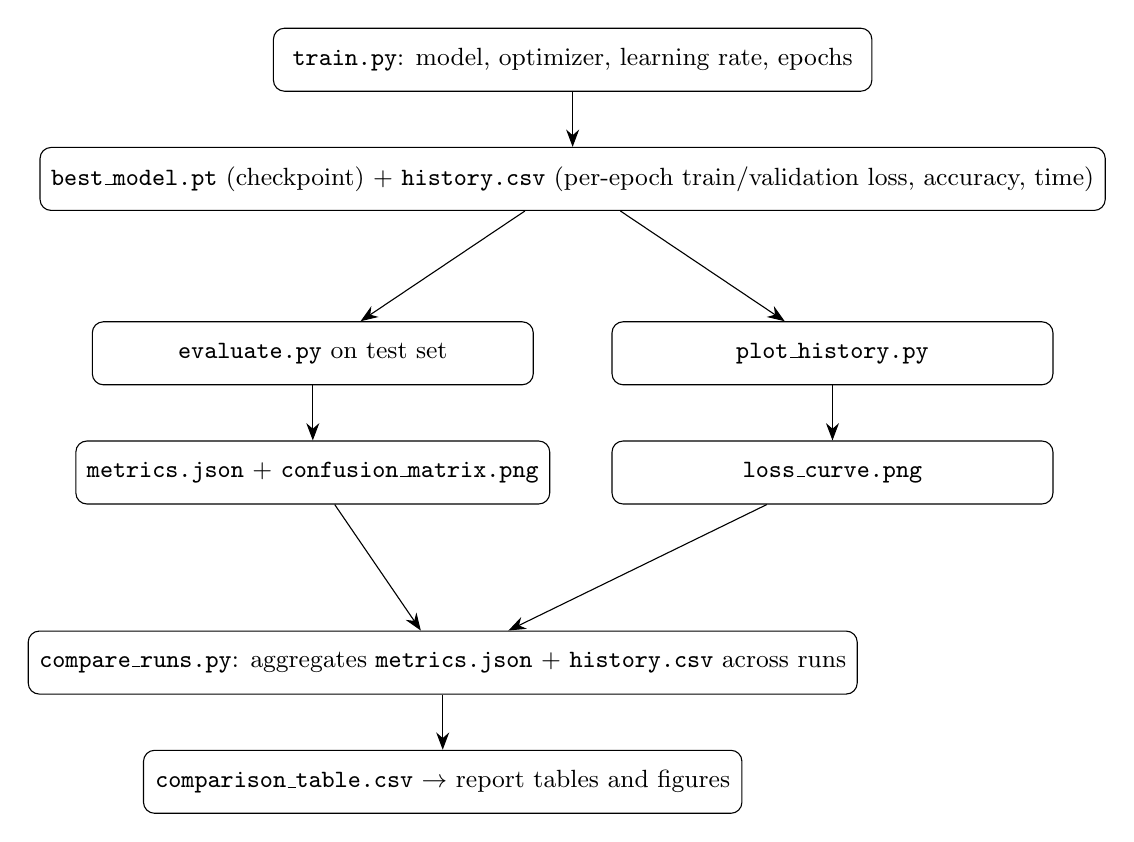
\begin{tikzpicture}[
  node distance=7mm and 10mm,
  box/.style={draw, rounded corners, align=center, font=\small,
    minimum height=8mm, inner sep=4pt},
  wide/.style={box, minimum width=7.6cm},
  narrow/.style={box, minimum width=5.6cm},
  arr/.style={-{Stealth[length=2.2mm]}}
]
\node[wide] (train) {\texttt{train.py}: model, optimizer, learning rate, epochs};
\node[wide, below=of train] (ckpt)
  {\texttt{best\_model.pt} (checkpoint) + \texttt{history.csv}
  (per-epoch train/validation loss, accuracy, time)};
\node[narrow, below=14mm of ckpt, xshift=-3.3cm] (eval)
  {\texttt{evaluate.py} on test set};
\node[narrow, below=14mm of ckpt, xshift=3.3cm] (plot)
  {\texttt{plot\_history.py}};
\node[narrow, below=of eval] (evalout)
  {\texttt{metrics.json} + \texttt{confusion\_matrix.png}};
\node[narrow, below=of plot] (plotout)
  {\texttt{loss\_curve.png}};
\node[wide, below=16mm of evalout, xshift=1.65cm] (compare)
  {\texttt{compare\_runs.py}: aggregates \texttt{metrics.json} +
  \texttt{history.csv} across runs};
\node[wide, below=of compare] (table)
  {\texttt{comparison\_table.csv} $\rightarrow$ report tables and figures};

\draw[arr] (train) -- (ckpt);
\draw[arr] (ckpt) -- (eval);
\draw[arr] (ckpt) -- (plot);
\draw[arr] (eval) -- (evalout);
\draw[arr] (plot) -- (plotout);
\draw[arr] (evalout) -- (compare);
\draw[arr] (plotout) -- (compare);
\draw[arr] (compare) -- (table);
\end{tikzpicture}%
}
\caption{Training, evaluation, and comparison pipeline shared by the four
reported models.}
\label{fig:training-pipeline}
\end{figure}

\subsection{Loss curves}

\begin{figure}[H]
\centering
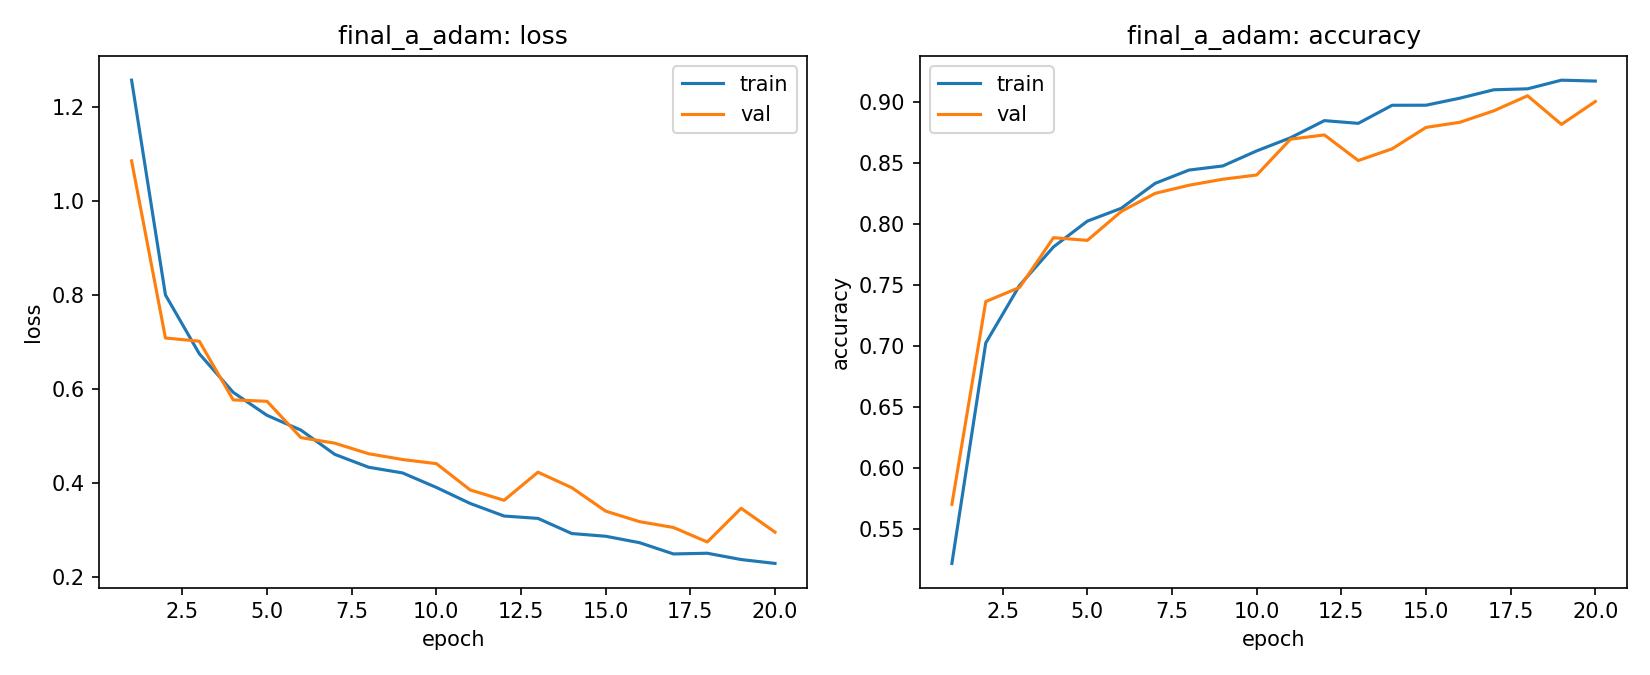
\includegraphics[width=0.85\textwidth]{figures/model_a_loss_curve.png}
\caption{Model A training/validation loss and accuracy vs. epoch.}
\label{fig:model-a-loss}
\end{figure}

\begin{figure}[H]
\centering
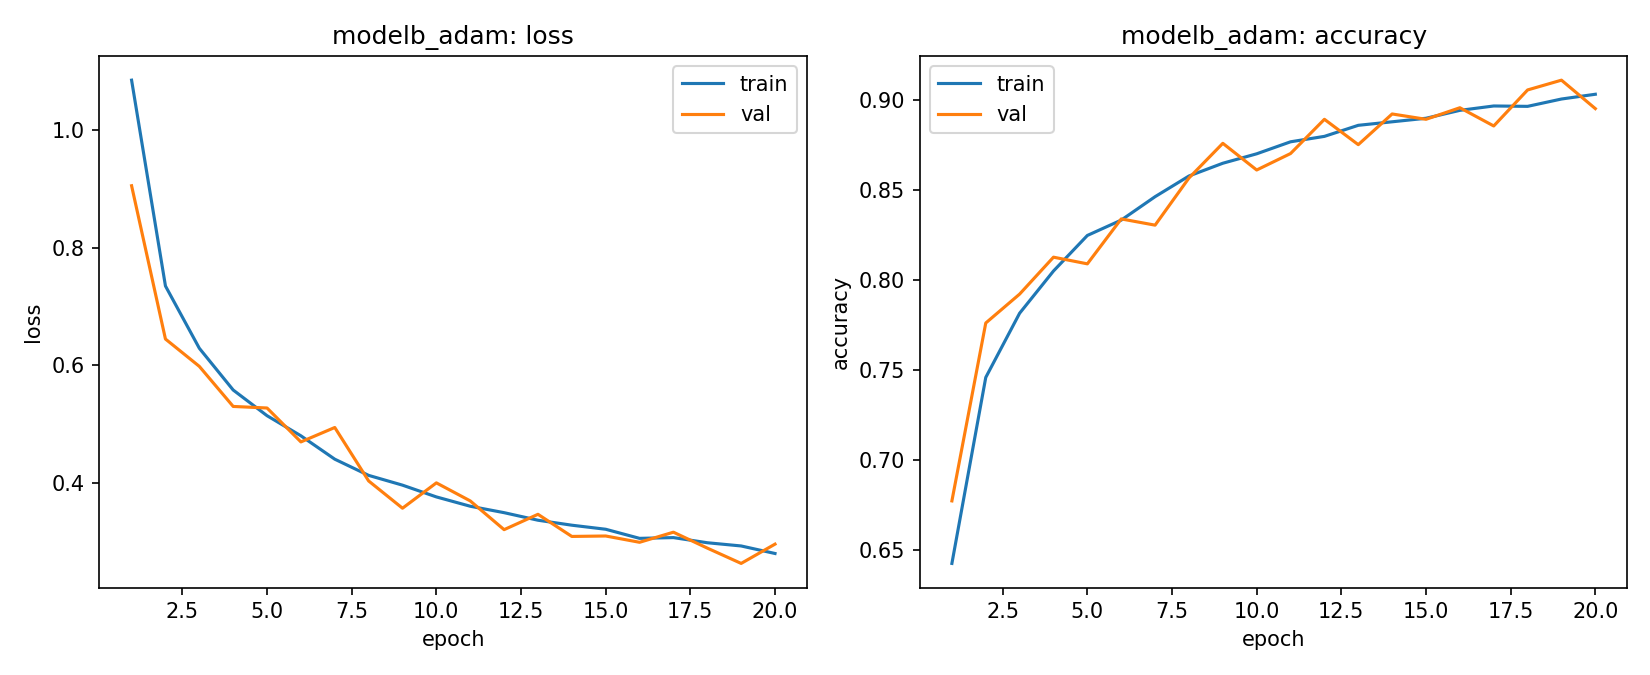
\includegraphics[width=0.85\textwidth]{figures/model_b_loss_curve.png}
\caption{Model B training/validation loss and accuracy vs. epoch.}
\label{fig:model-b-loss}
\end{figure}

Model A's training and validation curves (Figure~\ref{fig:model-a-loss})
track closely for roughly the first 11 epochs, after which a gap opens: by
epoch 20, training accuracy reaches $92.0\%$ while validation accuracy
peaks at $89.4\%$ ($88.1\%$ at epoch 20). This is a mild overfitting
signal, consistent with the architectural observation from
Section~\ref{sec:custom-models} that Model A's $524{,}416$  parameter FC1
layer ($95.5\%$ of all parameters) has no dropout, weight decay, or batch
normalization to regularize it. Model B's curves
(Figure~\ref{fig:model-b-loss}) show no such late-training divergence,
reaching $90.4\%$ training accuracy and $91.1\%$ peak validation accuracy,
because its batch normalization layers and global average pooling head
provide effective structural regularization while leaving far fewer
parameters available to overfit.

\subsection{Confusion matrices and per class metrics}

\begin{figure}[H]
\centering
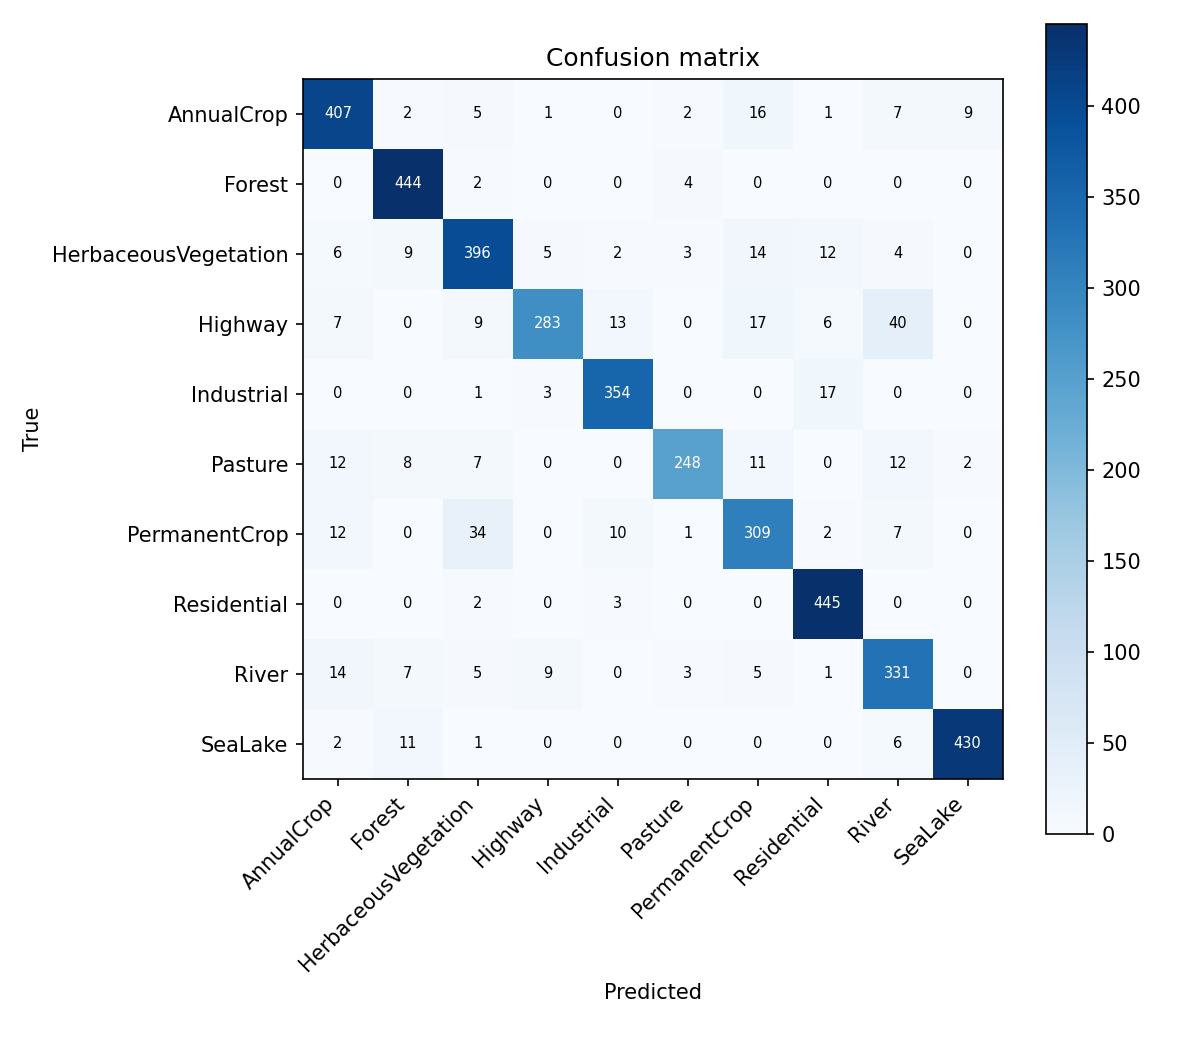
\includegraphics[width=0.72\textwidth]{figures/model_a_confusion_matrix.png}
\caption{Model A confusion matrix (test set).}
\label{fig:model-a-cm}
\end{figure}

\begin{figure}[H]
\centering
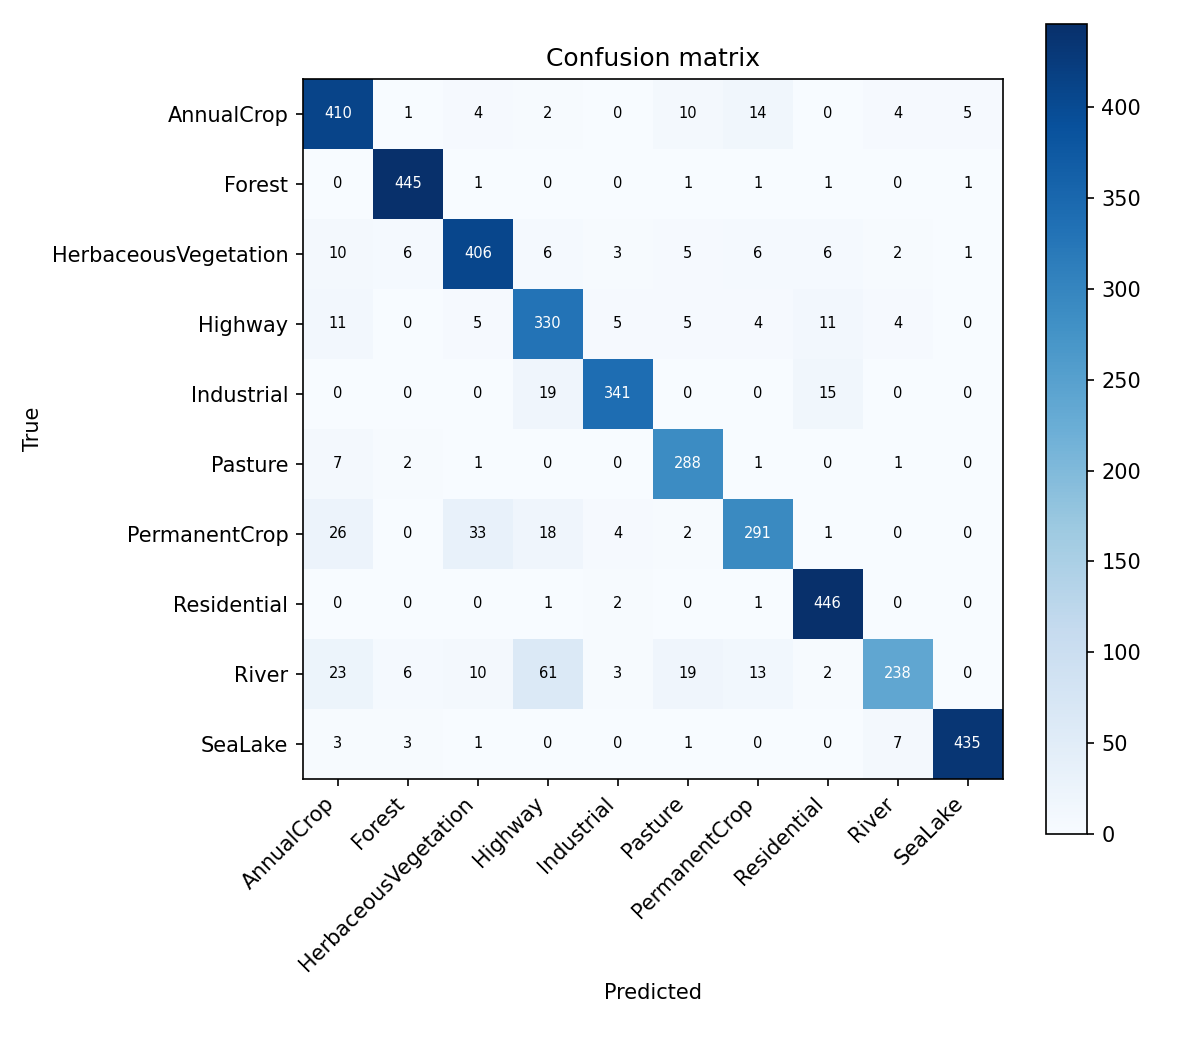
\includegraphics[width=0.72\textwidth]{figures/model_b_confusion_matrix.png}
\caption{Model B confusion matrix (test set).}
\label{fig:model-b-cm}
\end{figure}

\begin{table}[H]
\centering
\caption{Per class precision and recall on the test set, Model A vs. Model B.}
\label{tab:per-class-ab}
\begin{tabular}{lrrrr}
\toprule
 & \multicolumn{2}{c}{Model A} & \multicolumn{2}{c}{Model B} \\
Class & Precision & Recall & Precision & Recall \\
\midrule
AnnualCrop            & 0.885 & 0.904 & 0.880 & 0.909 \\
Forest                & 0.923 & 0.987 & 0.971 & 0.978 \\
HerbaceousVegetation  & 0.857 & 0.878 & 0.858 & 0.925 \\
Highway               & 0.940 & 0.755 & 0.925 & 0.789 \\
Industrial            & 0.927 & 0.944 & 0.908 & 0.976 \\
Pasture               & 0.950 & 0.827 & 0.903 & 0.903 \\
PermanentCrop         & 0.831 & 0.824 & 0.823 & 0.829 \\
Residential           & 0.919 & 0.989 & 0.975 & 0.962 \\
River                 & 0.813 & 0.883 & 0.853 & 0.837 \\
SeaLake               & 0.975 & 0.956 & 0.991 & 0.956 \\
\midrule
\textbf{Macro average} & \textbf{0.902} & \textbf{0.895} & \textbf{0.909} & \textbf{0.906} \\
\bottomrule
\end{tabular}
\end{table}

Both models share the same two hardest confusion pairs:
\textbf{Highway$\leftrightarrow$River} (both thin, elongated, linear
features at this resolution) and \textbf{HerbaceousVegetation
$\leftrightarrow$ PermanentCrop} (overlapping crop/vegetation texture). These
are the lowest recall classes for both models, which suggests the confusion
is a genuine property of the dataset at $64\times64$ RGB resolution rather
than a weakness specific to either architecture.

\subsection{Comparison table}

\begin{table}[H]
\centering
\caption{Model A vs. Model B comparison (20 epochs, Adam, $\text{lr}=10^{-3}$, Tesla T4 GPU).}
\label{tab:ab-comparison}
\begin{tabular}{lrrrr}
\toprule
Model & Parameters & Checkpoint size & Median time/epoch & Test accuracy \\
\midrule
Model A (standard CNN) & 549{,}290 & 2{,}150.1 KB & 8.53 s & 90.03\% \\
Model B (depthwise-sep.) & 13{,}288 & 63.9 KB & 8.66 s & \textbf{91.01\%} \\
\bottomrule
\end{tabular}
\end{table}
\emph{Time/epoch is reported as the median across epochs on a dedicated Tesla T4 GPU, providing an exact, head to head wall clock comparison under identical cloud hardware.}

\subsection{Discussion: standard vs. depthwise separable trade offs}

Model B uses only $13{,}288 / 549{,}290 \approx 2.4\%$ of Model A's
parameters and produces a checkpoint roughly $34\times$ smaller
($63.9$~KB vs.\ $2{,}150.1$~KB), while actually \emph{outperforming} Model A
by $0.98$ percentage points ($91.01\%$ vs.\ $90.03\%$) on the test set. This is
a striking result for the depthwise separable design: by replacing the dense
$524{,}416$ parameter flatten+FC1 head with global average pooling and adding
batch normalization to each depthwise separable stage, Model B eliminates the
overfitting bottleneck of Model A while cutting the memory footprint by $97.0\%$.

When comparing wall clock training speed on the GPU, Model B's median epoch time
($8.66$~s) is nearly identical to Model A's ($8.53$~s). Despite having $97.6\%$ fewer
trainable parameters and $2.28\times$ fewer theoretical MAC operations ($5.14$~M vs.\ $11.73$~M), Model B does
not show a wall clock speedup on a desktop/datacenter GPU because grouped depthwise
convolutions have lower arithmetic intensity (FLOPs per byte transferred) compared to dense
convolutions, which fully saturate GPU tensor cores. On edge hardware with specialized
runtimes (such as TFLite with XNNPACK or mobile NPUs), the substantial reduction in total
operations and memory footprint allows Model B to execute efficiently within strict embedded
SRAM and Flash memory budgets where Model A would exceed available capacity.

\section{SOTA Fine-Tuning and Evaluation}
\label{sec:sota}

Two ImageNet-pretrained, mobile/edge oriented architectures were fine tuned
end to end on the same EuroSAT data splits and compliant $64\times64$ input
resolution used for the custom models:
\textbf{MobileNetV2} and \textbf{EfficientNet-B0}. For both, the final
ImageNet classification layer was replaced with a fresh
$\text{Linear}(\cdot \rightarrow 10)$ layer, and \emph{all} layers (not just
the new head) were fine-tuned, using Adam with $\text{lr}=10^{-4}$ (a lower
learning rate than the custom models, appropriate for not disturbing the
pretrained features too aggressively) for 5 epochs.

\begin{table}[H]
\centering
\caption{SOTA fine tuning results (5 epochs, Adam, $\text{lr}=10^{-4}$, $64\times64$, Tesla T4 GPU).}
\label{tab:sota-results}
\begin{tabular}{lrrrrrr}
\toprule
Model & Input & Params & Size (MB) & Median time/epoch & Test accuracy & Macro P / R \\
\midrule
MobileNetV2 & $64\times64$ & 2{,}236{,}682 & 8.77 & 12.45 s & \textbf{97.58\%} & 0.975 / 0.974 \\
EfficientNet-B0 & $64\times64$ & 4{,}020{,}358 & 15.62 & 16.39 s & 97.36\% & 0.973 / 0.972 \\
\bottomrule
\end{tabular}
\end{table}

\begin{figure}[H]
\centering
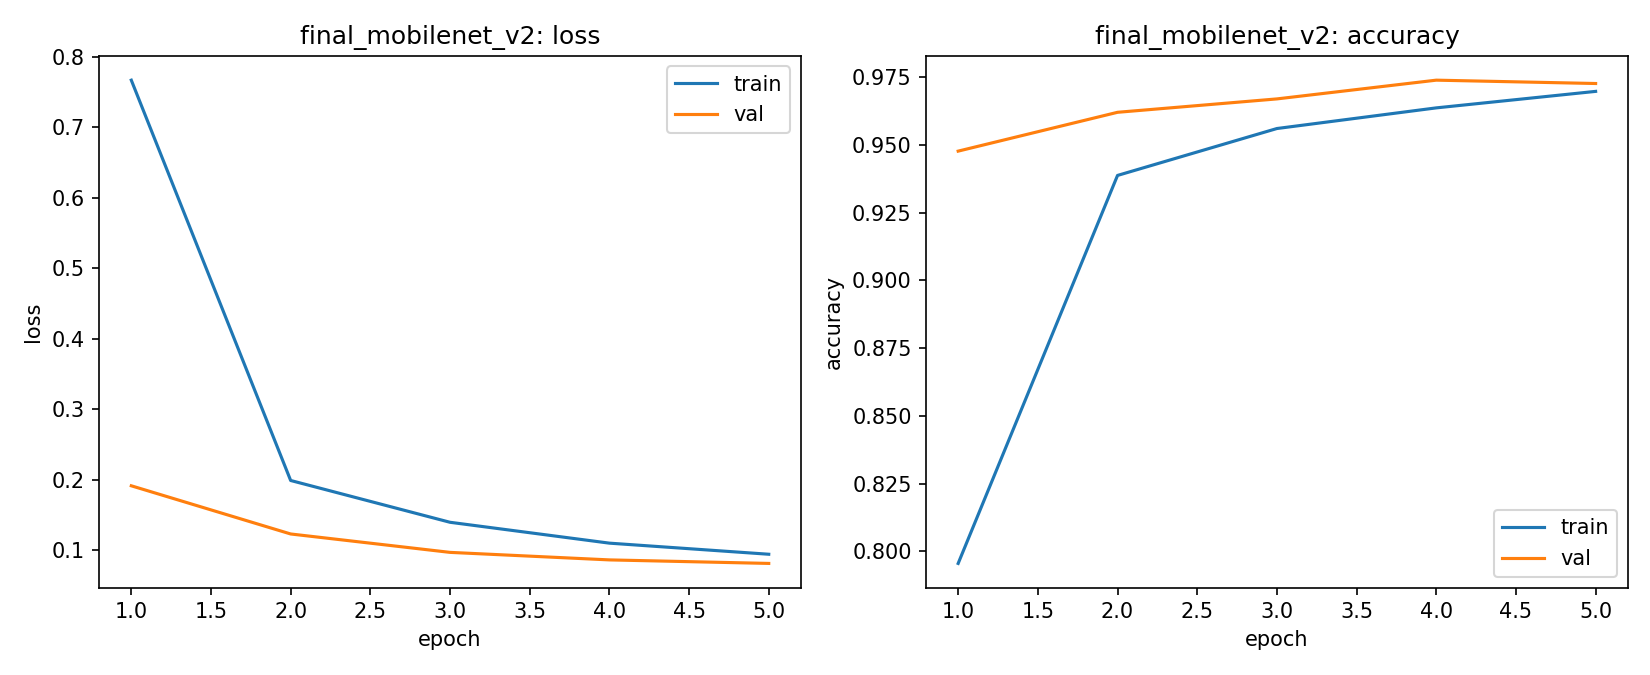
\includegraphics[width=0.85\textwidth]{figures/mobilenetv2_loss_curve.png}
\caption{MobileNetV2 ($64\times64$) fine tuning: training/validation loss and accuracy.}
\label{fig:mobilenetv2-loss}
\end{figure}

\begin{figure}[H]
\centering
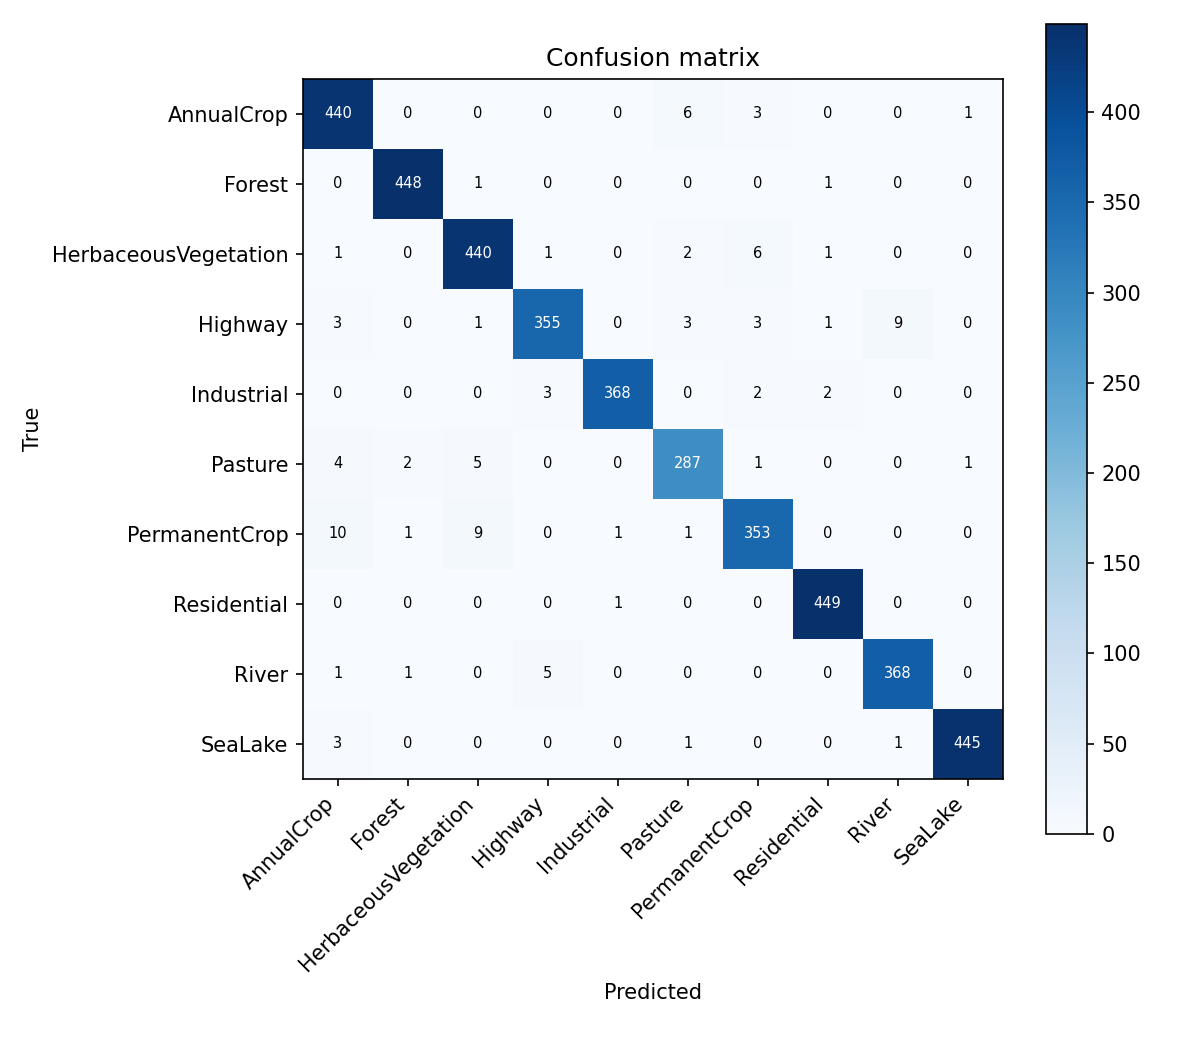
\includegraphics[width=0.72\textwidth]{figures/mobilenetv2_confusion_matrix.png}
\caption{MobileNetV2 ($64\times64$) confusion matrix (test set).}
\label{fig:mobilenetv2-cm}
\end{figure}

\begin{figure}[H]
\centering
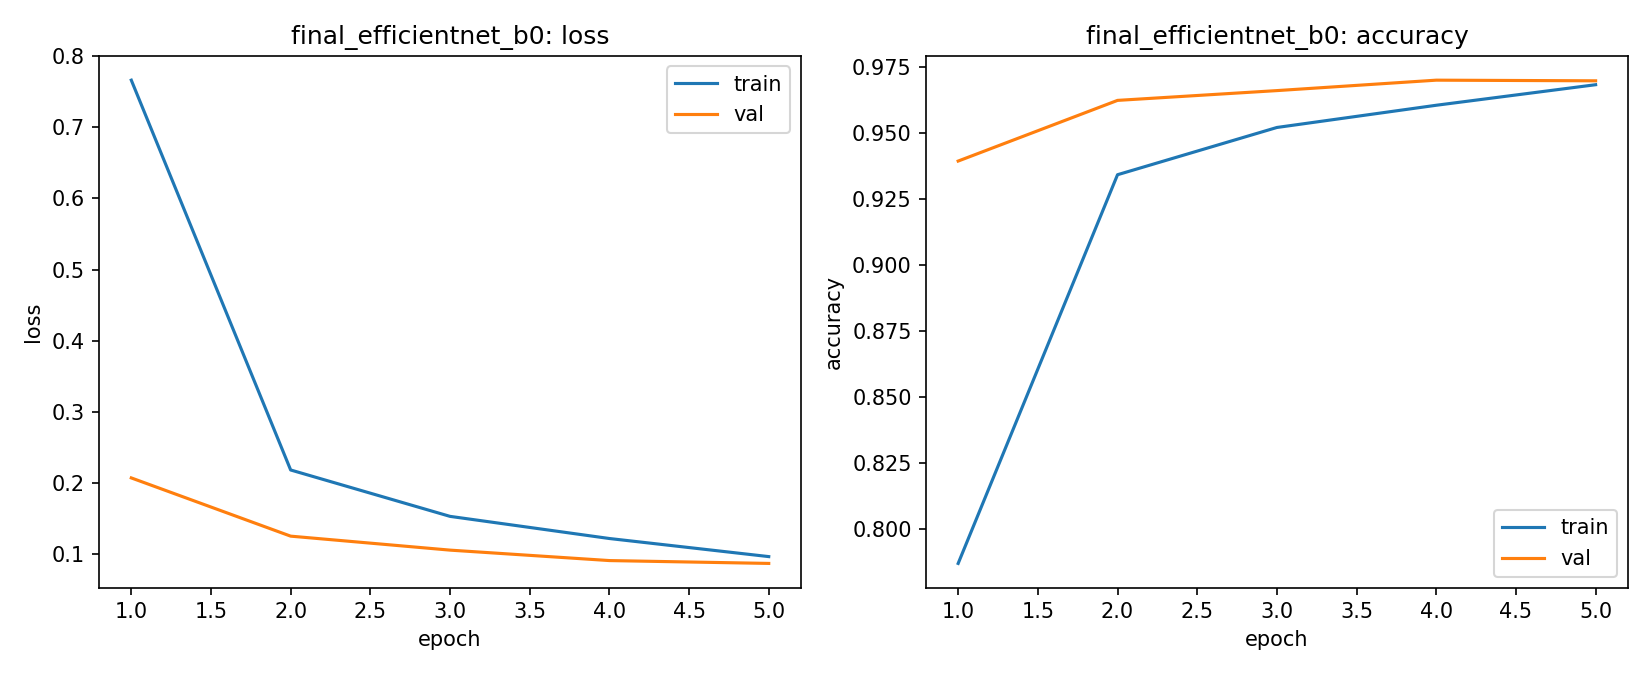
\includegraphics[width=0.85\textwidth]{figures/efficientnetb0_loss_curve.png}
\caption{EfficientNet-B0 ($64\times64$) fine tuning: training/validation loss and accuracy.}
\label{fig:effnet-loss}
\end{figure}

\begin{figure}[H]
\centering
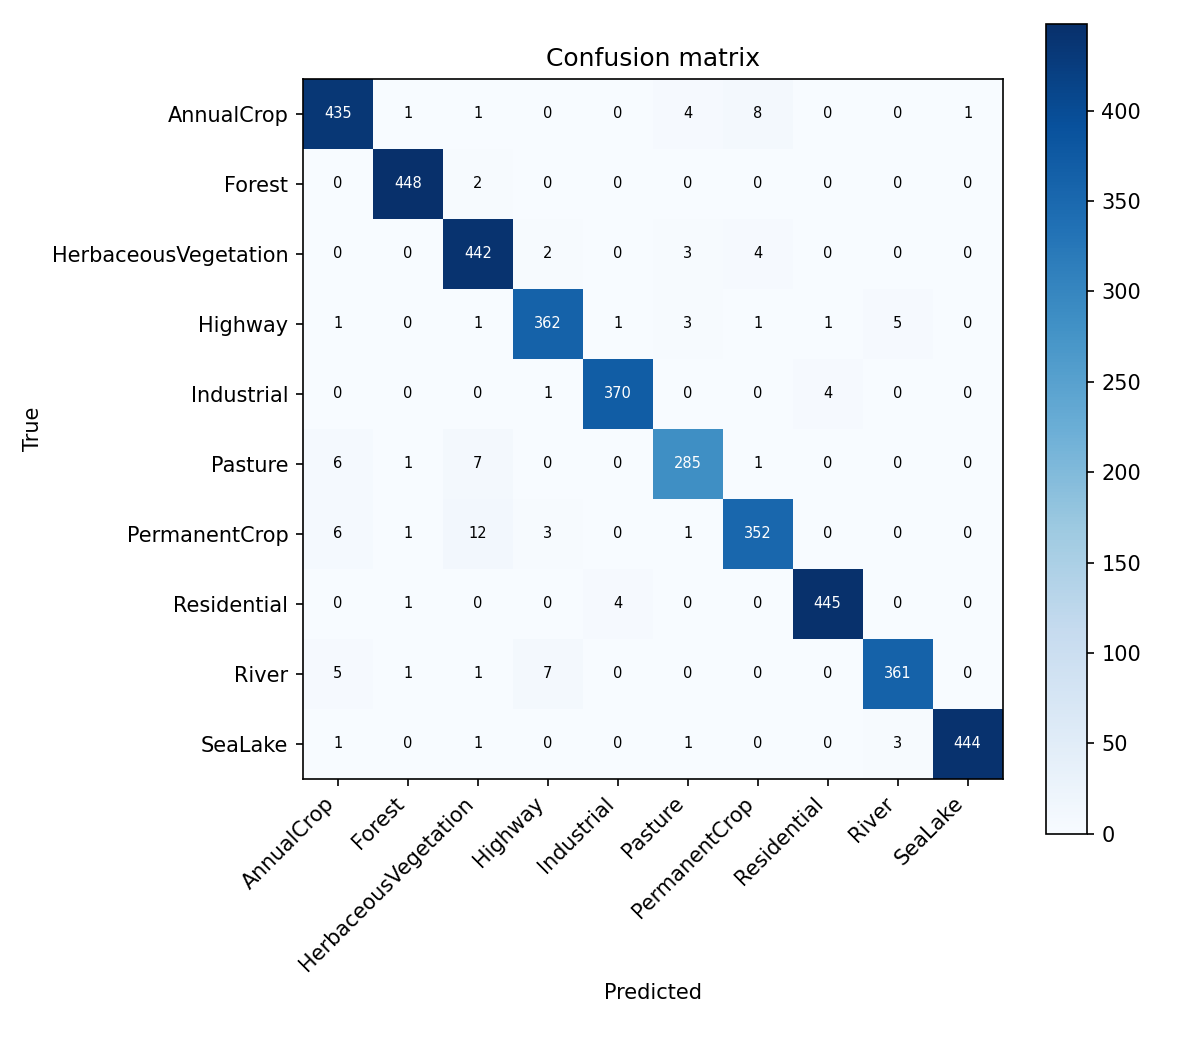
\includegraphics[width=0.72\textwidth]{figures/efficientnetb0_confusion_matrix.png}
\caption{EfficientNet-B0 ($64\times64$) confusion matrix (test set).}
\label{fig:effnet-cm}
\end{figure}

\begin{table}[H]
\centering
\caption{Per class precision and recall on the test set ($64\times64$), MobileNetV2 vs. EfficientNet-B0.}
\label{tab:per-class-sota}
\begin{tabular}{lrrrr}
\toprule
 & \multicolumn{2}{c}{MobileNetV2 ($64\times64$)} & \multicolumn{2}{c}{EfficientNet-B0 ($64\times64$)} \\
Class & Precision & Recall & Precision & Recall \\
\midrule
AnnualCrop            & 0.952 & 0.978 & 0.958 & 0.967 \\
Forest                & 0.991 & 0.996 & 0.989 & 0.996 \\
HerbaceousVegetation  & 0.965 & 0.976 & 0.946 & 0.980 \\
Highway               & 0.975 & 0.947 & 0.965 & 0.965 \\
Industrial            & 0.995 & 0.981 & 0.987 & 0.987 \\
Pasture               & 0.957 & 0.957 & 0.960 & 0.950 \\
PermanentCrop         & 0.959 & 0.941 & 0.962 & 0.939 \\
Residential           & 0.989 & 0.998 & 0.989 & 0.989 \\
River                 & 0.974 & 0.981 & 0.978 & 0.963 \\
SeaLake               & 0.996 & 0.989 & 0.998 & 0.987 \\
\midrule
\textbf{Macro average} & \textbf{0.975} & \textbf{0.974} & \textbf{0.973} & \textbf{0.972} \\
\bottomrule
\end{tabular}
\end{table}

Both fine tuned models comfortably exceed both custom models after only 5
epochs at the same $64\times64$ resolution expected, since they begin from
ImageNet pretrained features rather than random initialization. The same two
confusion pairs identified for the custom models (Highway/River,
HerbaceousVegetation/PermanentCrop) are still visible in
Figures~\ref{fig:mobilenetv2-cm} and~\ref{fig:effnet-cm}, but at far smaller
magnitude, reinforcing that these are genuinely hard classes for this dataset
at $64\times64$ resolution rather than an architecture specific weakness. At
equal $64\times64$ input resolution, MobileNetV2 ($97.58\%$) slightly edges
out EfficientNet B0 ($97.36\%$) while using roughly $44\%$ fewer parameters
and training $24\%$ faster per epoch ($12.45$~s vs.\ $16.39$~s).

\section{Final Comparison and Trade off Discussion}
\label{sec:final-comparison}

\begin{table}[H]
\centering
\caption{Final selected runs at $64\times64$ resolution: accuracy, memory, MACs, and relative footprint.}
\label{tab:final-comparison}
\begin{tabular}{lrrrrr}
\toprule
Model & Parameters & Size (MB) & Test accuracy & MACs (M) & Size vs.\ Model B \\
\midrule
Model A (custom, Adam) & 549{,}290 & 2.10 & 90.03\% & 11.73 & $\sim 34\times$ \\
Model B (custom, Adam) & 13{,}288 & 0.062 & 91.01\% & 5.14 & $1\times$ \\
MobileNetV2 (fine-tuned, $64\times64$) & 2{,}236{,}682 & 8.77 & 97.58\% & 24.46 & $\sim 141\times$ \\
EfficientNet-B0 (fine-tuned, $64\times64$) & 4{,}020{,}358 & 15.62 & 97.36\% & 31.98 & $\sim 252\times$ \\
\bottomrule
\end{tabular}
\end{table}

\paragraph{Accuracy.} The fine tuned SOTA models outperform Model B by
$6.35$--$6.57$ percentage points in test accuracy ($97.58\%$ and $97.36\%$ vs.\ $91.01\%$).
This gap is the direct benefit of transfer learning: both SOTA models started from features
learned on millions of ImageNet images, while Model B was trained entirely
from scratch on EuroSAT's 18{,}900 training images.

\paragraph{Memory footprint.} The gap here runs the other way, and far more
steeply: MobileNetV2's checkpoint is about $141\times$ larger than Model
B's, and EfficientNet-B0's is about $252\times$ larger. In absolute terms,
Model B's $63.9$~KB footprint ($92.6$~KB in TorchScript, $26.7$~KB graph in ONNX) is small enough to plausibly fit in the flash/RAM
of a microcontroller class device (e.g.\ typical Cortex-M class chips with
hundreds of KB to a few MB of flash), whereas both SOTA models' $8.8$--$15.6$~MB
footprints exceed that budget by two to three orders of magnitude and would
only be viable on richer edge hardware (e.g.\ a Raspberry Pi, a phone, or a
device with a dedicated NPU and MB-scale memory).

\paragraph{Activation memory: parameters are not the whole story.} Table~\ref{tab:final-comparison}
measures memory with stored weights alone, but peak RAM during inference is
dominated by the largest live feature maps, not the parameter count. For
Model A, the largest activation occurs at the first convolution: a
$16\times64\times64$ output (65{,}536 values) held alongside the
$3\times64\times64$ input (12{,}288 values), approximately 77{,}824 values
in total. For Model B, the first depthwise-separable block is \emph{wider}
(32 output channels, chosen to give the network enough capacity after
removing Model A's large dense head) and produces a $32\times64\times64$
pointwise output (131{,}072 values) alongside the same input, approximately
143{,}360 values in total -- roughly $1.8\times$ \emph{more} peak activation
memory than Model A, despite Model B having $97.6\%$ fewer parameters. In
float32 this is about $304$~KB (Model A) vs.\ $560$~KB (Model B); after INT8
quantization, approximately $76$~KB vs.\ $140$~KB (analytic estimate from
tensor shapes, excluding interpreter/runtime overhead). This is a useful
counterpoint to the headline parameter-count comparison: Model B's advantage
is in \emph{stored weight} footprint, not necessarily in peak working
memory, and a microcontroller target would need to budget SRAM for both
figures, not just the checkpoint size.

\paragraph{Computational cost.} The final table includes theoretical
convolution and linear MAC estimates at $64\times64$. Indicative synthetic
batch-one latency on the Kaggle benchmark machine was $0.41$~ms GPU / $1.20$~ms CPU (Model A),
$0.62$~ms GPU / $2.40$~ms CPU (Model B), $4.92$~ms GPU / $7.70$~ms CPU (MobileNetV2), and
$7.59$~ms GPU / $10.86$~ms CPU (EfficientNet-B0).
These measurements use newly initialized models and synthetic inputs, not
trained checkpoints, and are not physical edge device measurements. The MAC
profiler excludes normalization, activation, pooling, and other overhead.
Fine-tuning the SOTA models required far
fewer epochs to reach high accuracy (5 vs.\ 20 for the custom models),
reflecting the sample efficiency of transfer learning. However, each SOTA
epoch was computationally heavier: on the Tesla T4 GPU at $64\times64$, MobileNetV2 required
$12.45$~s per epoch and EfficientNet-B0 required $16.39$~s per epoch,
compared to Model B's $8.66$~s per epoch. Inference-time results depend heavily on the deployment hardware's support for
standard vs.\ depthwise-separable/grouped convolution kernels.

\paragraph{Recommendation.} The choice between a custom sub 100k parameter
model and a fine-tuned SOTA model is fundamentally a question of \emph{where
in the accuracy memory compute space the target hardware sits}:
\begin{itemize}
  \item For the tightest microcontroller class targets (KB scale memory, no
  practical way to download or store multi MB weights), Model B is the only
  one of the three options that is even feasible, and its $91.01\%$
  accuracy is a strong result for that constraint.
  \item For richer edge devices with MB-scale memory and reasonable compute
  (Raspberry Pi class hardware, phones, edge accelerators), the
  $6.4$--$6.6$ percentage point accuracy improvement from a fine tuned SOTA
  model is substantial and, given the available memory headroom, likely
  worth the larger footprint : particularly since production inference
  runtimes (e.g.\ TFLite/XNNPACK, mobile NPUs) are specifically optimized
  for depthwise separable operations and would likely close or reverse the
  CPU training time gap observed in this assignment's unoptimized training
  environment.
  \item There is no universally "better" choice among the three models;
  the right one depends entirely on the deployment target's memory budget
  and the accuracy requirement of the application.
\end{itemize}

\section{Limitations and Threats to Validity}
\label{sec:limitations}

\begin{itemize}
  \item \textbf{Single run per configuration.} Each model/optimizer
  combination was trained once with a fixed seed (42). The $0.98$
  percentage point gap between Model A and Model B, and the $0.22$ point
  gap between MobileNetV2 and EfficientNet-B0, are within the range that a
  different random initialization could plausibly change; no confidence
  intervals or repeated-seed statistics were computed.
  \item \textbf{Inconsistent hardware for the optimizer sweep.} The Model A
  optimizer sweep (Section~\ref{sec:optimizer}, Table~\ref{tab:model-a-sweep})
  was run on local CPU hardware before the project migrated to a Kaggle
  Tesla T4 GPU for all other reported numbers. Its qualitative conclusion
  (SGD with momentum closes most of the gap to Adam) is corroborated by the
  full-length, Tesla T4 Model B run in Table~\ref{tab:model-b-optimizer},
  but the absolute numbers in that one table are not on the same hardware
  basis as the rest of the report.
  \item \textbf{Limited SOTA hyperparameter search.} Both pretrained models
  were fine-tuned with a single fixed recipe (Adam, $\text{lr}=10^{-4}$, 5
  epochs) rather than a tuned schedule; a learning-rate sweep or more epochs
  might change the ranking between MobileNetV2 and EfficientNet-B0.
  \item \textbf{Synthetic, untrained-model benchmarks.} The MAC/FLOP and
  latency figures in Table~\ref{tab:final-comparison} and
  Section~\ref{sec:final-comparison} are measured on newly initialized
  models with synthetic inputs, not the trained checkpoints, and exclude
  normalization/activation/pooling overhead. They are not physical
  edge-device measurements and should be treated as indicative only.
  \item \textbf{No quantized or on-device evaluation.} TorchScript and ONNX
  export were verified for numerical parity with the PyTorch checkpoints,
  but no INT8 quantization or actual microcontroller/edge-board latency
  measurement was performed; the "fits on a microcontroller" claims for
  Model B (Section~\ref{sec:final-comparison}) are based on checkpoint size
  and the activation-memory estimate above, not a measured deployment.
  \item \textbf{Dataset realism.} EuroSAT is a curated, largely cloud-free
  Sentinel-2 benchmark; a real edge sensor (e.g.\ an onboard satellite or
  drone camera) would additionally face atmospheric effects, sensor noise,
  and viewing-angle variation not represented here, so reported accuracies
  should be read as an upper bound relative to a genuinely deployed system.
  \item \textbf{Persistent class confusions.} Even the best-performing
  fine-tuned models do not fully resolve the Highway/River and
  HerbaceousVegetation/PermanentCrop confusions identified in
  Section~\ref{sec:custom-training}; this appears to be a
  resolution/dataset limit rather than something further training of these
  particular architectures would fix.
\end{itemize}

\section{Conclusion}

This assignment implemented and evaluated two custom CNNs (a standard
549{,}290 parameter model and a 13{,}288 parameter depthwise separable
model, $97.6\%$ smaller) and two fine tuned pretrained lightweight models
(MobileNetV2 and EfficientNet-B0) on the EuroSAT land use classification
task, with all four models trained and evaluated at the compliant $64\times64$
resolution on an identical 70/15/15 stratified split. Using the selected Adam
runs, Model A reached $90.03\%$ test accuracy and Model B reached $91.01\%$,
demonstrating that depthwise separable convolutions paired with batch
normalization and global average pooling can match or exceed a $41\times$ larger
standard CNN while fitting easily within a sub 100k parameter budget. The
two fine tuned SOTA models reached $97.58\%$ (MobileNetV2) and $97.36\%$
(EfficientNet-B0) at $64\times64$ resolution at the cost of $141$--$252\times$
larger checkpoint footprints. These results illustrate the classic
accuracy vs footprint trade off that governs edge deployment model
selection: the "best" model depends on where the target hardware sits on
that spectrum, not on a single universal accuracy ranking.

\begin{thebibliography}{9}
\bibitem{eurosat}
P.~Helber, B.~Bischke, A.~Dengel, and D.~Borth, ``EuroSAT: A Novel Dataset
and Deep Learning Benchmark for Land Use and Land Cover Classification,''
\emph{IEEE Journal of Selected Topics in Applied Earth Observations and
Remote Sensing}, 2019.

\bibitem{mobilenetv2}
M.~Sandler, A.~Howard, M.~Zhu, A.~Zhmoginov, and L.-C.~Chen, ``MobileNetV2:
Inverted Residuals and Linear Bottlenecks,'' \emph{CVPR}, 2018.

\bibitem{efficientnet}
M.~Tan and Q.~V.~Le, ``EfficientNet: Rethinking Model Scaling for
Convolutional Neural Networks,'' \emph{ICML}, 2019.

\bibitem{adam}
D.~P.~Kingma and J.~Ba, ``Adam: A Method for Stochastic Optimization,''
\emph{ICLR}, 2015.

\bibitem{lecun1998}
Y.~LeCun, L.~Bottou, Y.~Bengio, and P.~Haffner, ``Gradient-based learning
applied to document recognition,'' \emph{Proceedings of the IEEE}, vol.~86,
no.~11, pp.~2278--2324, 1998.

\end{thebibliography}

\end{document}
